\subsubsection{WikiSQL Dataset}

WikiSQL consists of 80K+ natural language questions and corresponding SQL queries on 24K+ tables extracted from Wikipedia. Neither the train nor development sets contain the database in the test set. Databases and SQL queries have simplified the dataset's creators' assumptions. This dataset consists only of SQL labels covering a single SELECT column and aggregation and WHERE conditions. Furthermore, all the databases contain only one table.

The database does not include complex queries involving advanced operations like JOIN, GROUP BY, ORDER BY, etc. Prior to the release of SPIDER, this dataset was considered to be a benchmark dataset. Using WikiSQL has been the subject of a great deal of research. WikiSQL's "WHERE" clause has been recognized as one of the most challenging clauses to parse semantically, and SQLNet and SyntaxSQL were previous state-of-the-art models.


\begin{figure}[htb]
    \centering
    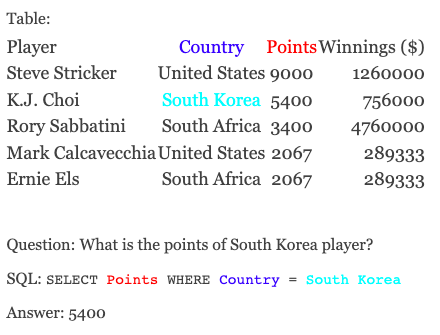
\includegraphics[width=0.5\textwidth]{pics/db/WikiSQL.png}
    \caption{Example from WikiSQL dataset\cite{DBLP:journals/corr/abs-1902-01069}}
    \label{fig:WikiSQL}
\end{figure}

The WikiSQL challenge is a research competition focused on developing natural language interfaces for databases. The challenge includes several state-of-the-art Text-to-SQL solutions proposed by different research teams.

One example of a state-of-the-art Text-to-SQL solution in the WikiSQL challenge is the Seq2SQL model, which uses a sequence-to-sequence learning framework to map natural language input to SQL queries. The model uses an attention mechanism to align the input and output sequences and a pointer network to handle SQL queries with complex structural dependencies.

Another example is the Spider model, which uses a combination of recurrent and convolutional neural networks to learn the mapping between natural language and SQL queries. The model uses a hierarchical structure to process the natural language input, with separate modules for understanding the query's intent, columns, and constraints.
One difference between these research approaches is the specific deep learning architecture used. The Seq2SQL model uses a sequence-to-sequence framework, while the Spider model uses a combination of RNNs and convolutional neural networks. Additionally, the Spider model uses a hierarchical structure to process the natural language input, while the Seq2SQL model processes the input linearly.

Another difference is in the evaluation metrics used. The Seq2SQL model is evaluated using the execution accuracy of the generated SQL queries, while the Spider model is evaluated using a combination of execution accuracy and natural language understanding metrics.
Overall, both the Seq2SQL and Spider models are state-of-the-art Text-to-SQL solutions that have achieved high performance in the WikiSQL challenge. However, their specific architectures and evaluation metrics differ, which can affect their performance and accuracy on different tasks.
